\section{Zadania zrealizowane}

\subsection*{Front-end}
\begin{itemize}
  \item zrealizowana strona główna, dostępna dla użytkowników niezalogowanych,
  \item rozbudowany moduł administratora, zapewniający pełną obsługę użytkowników,
  \item zrealizowana strona rejestracji nowego użytkownika,
  \item strona rejestracji jest w pełni funkcjonalna, sprawdza wprowadzone wartości, jeśli są poprawne dodaje nowego użytkownika do bazy danych, 
  \item zrealizowana strona logowania,
  \item strona logowania zapewnia autentykację użytkownika, po wprowadzeniu błędnych danych wypisuje komunikat "Username or password is incorrect", po wprowadzeniu poprawnych danych przekierowuje do strony głównej, 
\end{itemize}

\subsection*{Back-end}
\begin{itemize}
  \item Tworzenie namespacu i uruchomianie procesu w namespace'ie 
  \item Obsługa openVPN z poziomu konsoli 
  \item Przekierowanie na interfejs openVPN ruchu z namespac'u 
  \item Obsługa zapytań do bazy danych z poziomu pythona
  \item Projekt struktury bazy danych
\end{itemize}

\newpage

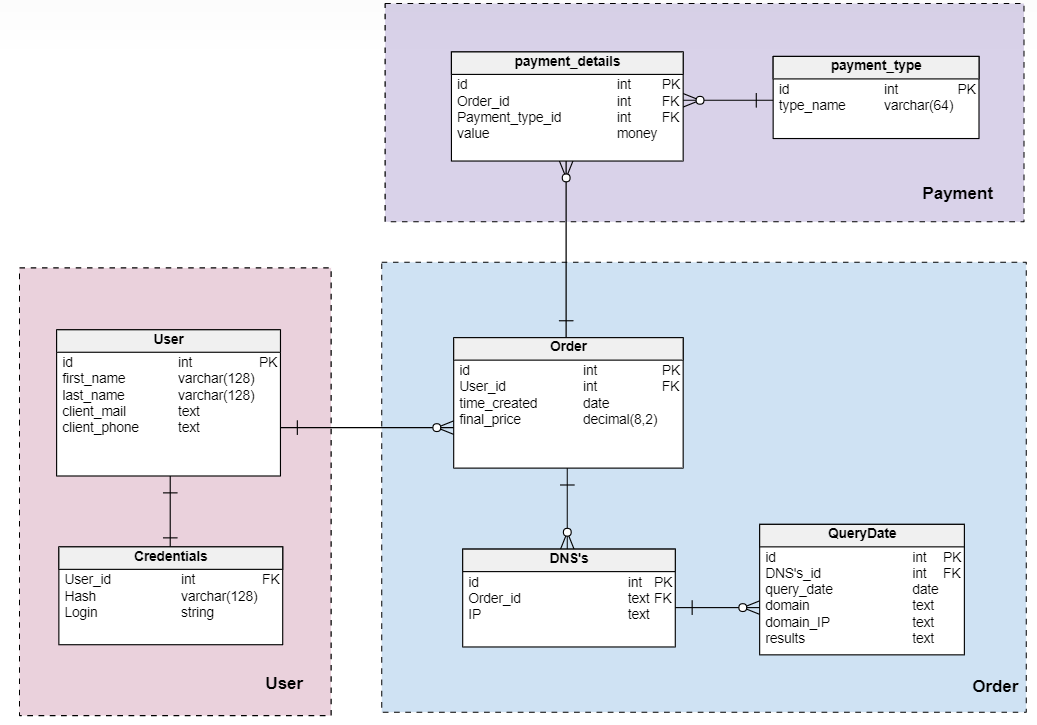
\includegraphics[scale=0.6]{db_schema.png}
